\section{¿Qué es el arco de un ángulo?}\label{sec:arcoangulo}

El arco de un ángulo en una circunferencia es la porción de la circunferencia que corresponde a ese ángulo central. Si el ángulo es $\theta$ (en radianes), el arco es la longitud que abarca sobre la circunferencia, y se calcula como:

\[
    L = r \theta
\]

donde $r$ es el radio de la circunferencia y $L$ es la longitud del arco.

En trigonometría, el concepto de arco también se usa para referirse a la función inversa de las funciones trigonométricas, como el arccoseno ($\arccos$), el arco seno ($\arcsin$) y el arco tangente ($\arctan$), que devuelven el ángulo cuyo coseno, seno o tangente es un valor dado.

Por ejemplo:
\begin{itemize}
    \item $\arccos(x)$ es el ángulo cuyo coseno es $x$.
    \item $\arcsin(x)$ es el ángulo cuyo seno es $x$.
    \item $\arctan(x)$ es el ángulo cuya tangente es $x$.
\end{itemize}

Así, el "arco de un ángulo" puede referirse tanto a la longitud sobre la circunferencia como a la función inversa en trigonometría.

\begin{center}
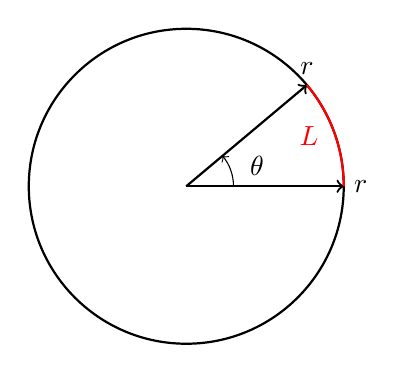
\begin{tikzpicture}[scale=2]
  % Circunferencia
  \draw[thick] (0,0) circle(1);
  % Radio inicial
  \draw[thick,->] (0,0) -- (1,0) node[anchor=west]{$r$};
  % Radio final
  \draw[thick,->] (0,0) -- ({cos(40)},{sin(40)}) node[anchor=south]{$r$};
  % Arco
  \draw[red,thick] (1,0) arc (0:40:1);
  % Ángulo
  \draw[->] (0.3,0) arc (0:40:0.3);
  \node at (0.45,0.13) {$\theta$};
  % Etiqueta del arco
  \node[red] at (0.78,0.32) {$L$};
\end{tikzpicture}
\end{center}
